\section{Scalability}
\label{app:scalability}
When scaling up the default ViT architecture, we encountered training instability in ViT at Adam $1e^{-3}$. Initially, the loss would decrease as normal, but within 2000 steps the loss steadily increased. \cref{fig:stability_8b} shows the behavior of attention logits during training for an 8B parameter model. Without normalization, attention logits quickly grow to over $50000$ in magnitude, resulting in one-hot attention weights after the softmax, and subsequently unstable training losses and gradients.

To avoid instability, the learning rate of ViT was originally reduced with increasing model scale, from 1e-3 down to 4e-4 for ViT-H~\citep{dosovitskiy2020image}. We retrain models up to ViT-L, comparing models trained similar to ViT, to models which have the normalization/reduced precision. For the latter, the learning rate is kept at 1e-3 and not reduced for larger models. With the QK-normalization, the higher 1e-3 learning rate remains stable. The results, shown in~\cref{fig:arch_sweep}, demonstrate increasing benefits with scale, likely due to enabling the larger learning rate.

\begin{figure}[htb]
    \centering
    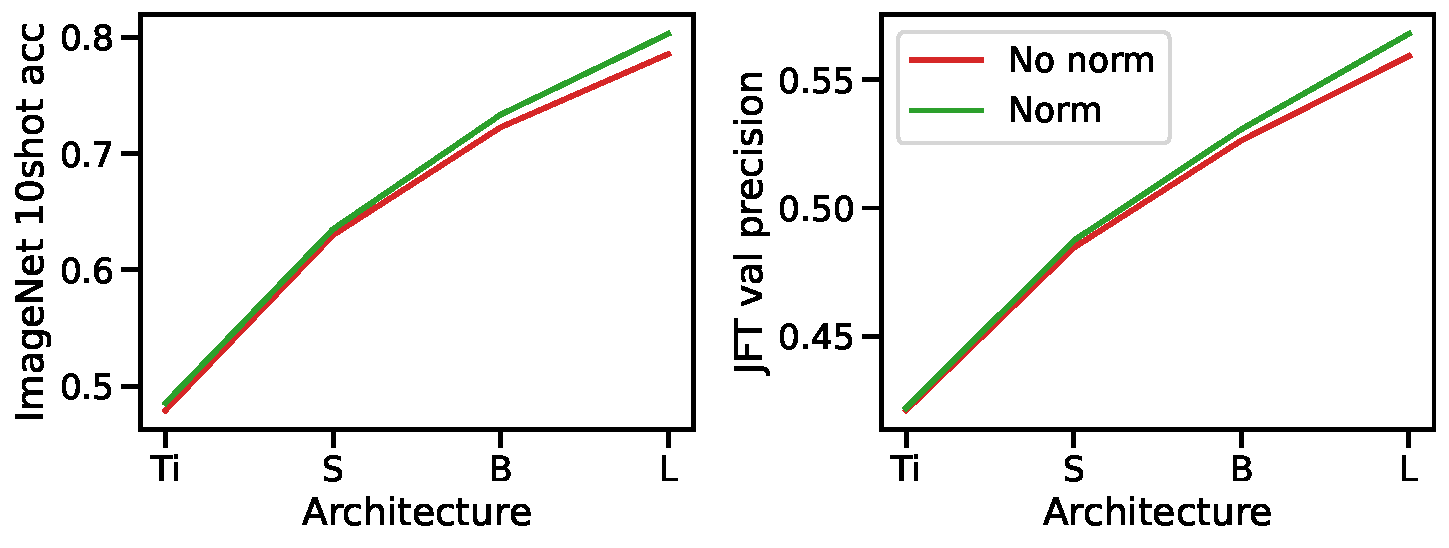
\includegraphics[width=0.7\columnwidth]{figs/arch_sweep.pdf}
    % \vspace{-10pt}
    \caption{Training models with and without query/key normalization; those that do not have normalization are trained with lower learning rates at larger scale, whereas those with normalization have a consistent learning rate of 1e-3.}
    \label{fig:arch_sweep}
\end{figure}